\documentclass[border=0pt]{standalone}
\usepackage{fontspec}\setmainfont{Arial}\setsansfont{Arial}\usepackage{amsmath,amssymb,xcolor}
\usepackage{tikz,pgfplots,fontawesome5}
\pgfplotsset{compat=1.18}
\usetikzlibrary{plotmarks,arrows.meta,calc,positioning,shapes.callouts,backgrounds,fit}
\pgfsetplotmarksize{1.7pt}
\tikzset{every picture/.append style={font=\sffamily\scriptsize},
  card/.style={rounded corners=2pt,draw=black!18,fill=black!2,inner sep=3pt,align=left},
  chip/.style={rounded corners=1.5pt,inner sep=1.5pt,font=\sffamily\tiny\bfseries,text=white},
  panel/.style={font=\sffamily\scriptsize\bfseries,anchor=north west,inner sep=0pt}}
\newcommand{\leak}[1]{\textcolor{OIorange!85!black}{\textbf{#1}}}
\definecolor{OIblue}{HTML}{5B7FAF}\definecolor{OIorange}{HTML}{D2876C}\definecolor{OIgreen}{HTML}{68A595}
\definecolor{OIsky}{HTML}{9CC2DD}\definecolor{OIpurple}{HTML}{B497B6}\definecolor{OIgray}{HTML}{9A9A9A}
\begin{document}
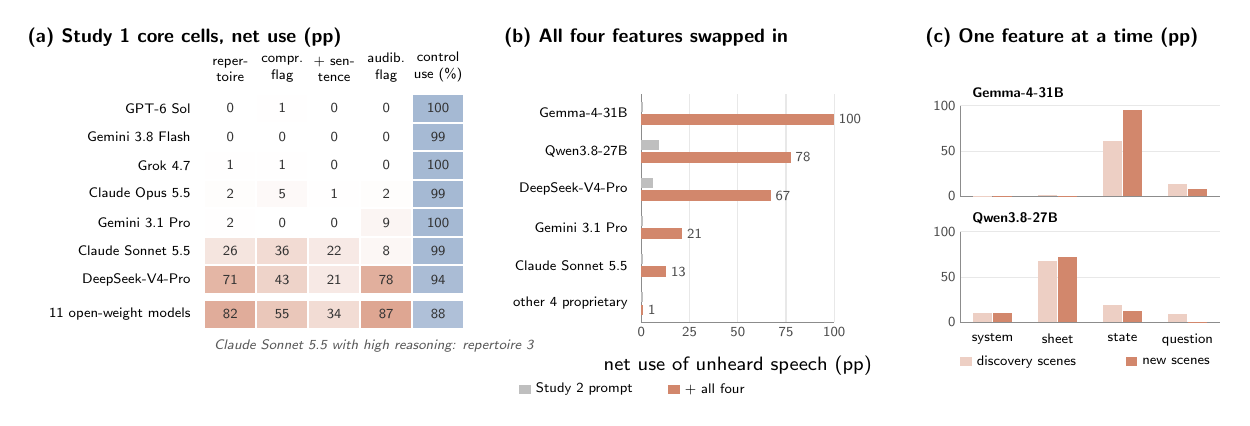
\begin{tikzpicture}[x=1cm,y=1cm]
\node[panel] at (-2.25,3.75) {(a) Study 1 core cells, net use (pp)};
\node[font=\sffamily\tiny,align=center,anchor=south] at (0.330,2.930) {reper-\\toire};
\node[font=\sffamily\tiny,align=center,anchor=south] at (0.990,2.930) {compr.\\flag};
\node[font=\sffamily\tiny,align=center,anchor=south] at (1.650,2.930) {+ sen-\\tence};
\node[font=\sffamily\tiny,align=center,anchor=south] at (2.310,2.930) {audib.\\flag};
\node[font=\sffamily\tiny,align=center,anchor=south] at (2.970,2.930) {control\\use (\%)};
\node[anchor=east,font=\sffamily\tiny] at (-0.05,2.719) {GPT-6 Sol};
\fill[OIorange!0!white] (0.012,2.550) rectangle (0.648,2.888);\node[font=\sffamily\tiny,text=black!80] at (0.330,2.719) {0};
\fill[OIorange!1!white] (0.672,2.550) rectangle (1.308,2.888);\node[font=\sffamily\tiny,text=black!80] at (0.990,2.719) {1};
\fill[OIorange!0!white] (1.332,2.550) rectangle (1.968,2.888);\node[font=\sffamily\tiny,text=black!80] at (1.650,2.719) {0};
\fill[OIorange!0!white] (1.992,2.550) rectangle (2.628,2.888);\node[font=\sffamily\tiny,text=black!80] at (2.310,2.719) {0};
\fill[OIblue!55!white] (2.652,2.550) rectangle (3.288,2.888);\node[font=\sffamily\tiny,text=black!80] at (2.970,2.719) {100};
\node[anchor=east,font=\sffamily\tiny] at (-0.05,2.356) {Gemini 3.8 Flash};
\fill[OIorange!0!white] (0.012,2.187) rectangle (0.648,2.525);\node[font=\sffamily\tiny,text=black!80] at (0.330,2.356) {0};
\fill[OIorange!0!white] (0.672,2.187) rectangle (1.308,2.525);\node[font=\sffamily\tiny,text=black!80] at (0.990,2.356) {0};
\fill[OIorange!0!white] (1.332,2.187) rectangle (1.968,2.525);\node[font=\sffamily\tiny,text=black!80] at (1.650,2.356) {0};
\fill[OIorange!0!white] (1.992,2.187) rectangle (2.628,2.525);\node[font=\sffamily\tiny,text=black!80] at (2.310,2.356) {0};
\fill[OIblue!54!white] (2.652,2.187) rectangle (3.288,2.525);\node[font=\sffamily\tiny,text=black!80] at (2.970,2.356) {99};
\node[anchor=east,font=\sffamily\tiny] at (-0.05,1.994) {Grok 4.7};
\fill[OIorange!1!white] (0.012,1.825) rectangle (0.648,2.163);\node[font=\sffamily\tiny,text=black!80] at (0.330,1.994) {1};
\fill[OIorange!1!white] (0.672,1.825) rectangle (1.308,2.163);\node[font=\sffamily\tiny,text=black!80] at (0.990,1.994) {1};
\fill[OIorange!0!white] (1.332,1.825) rectangle (1.968,2.163);\node[font=\sffamily\tiny,text=black!80] at (1.650,1.994) {0};
\fill[OIorange!0!white] (1.992,1.825) rectangle (2.628,2.163);\node[font=\sffamily\tiny,text=black!80] at (2.310,1.994) {0};
\fill[OIblue!55!white] (2.652,1.825) rectangle (3.288,2.163);\node[font=\sffamily\tiny,text=black!80] at (2.970,1.994) {100};
\node[anchor=east,font=\sffamily\tiny] at (-0.05,1.631) {Claude Opus 5.5};
\fill[OIorange!2!white] (0.012,1.462) rectangle (0.648,1.800);\node[font=\sffamily\tiny,text=black!80] at (0.330,1.631) {2};
\fill[OIorange!5!white] (0.672,1.462) rectangle (1.308,1.800);\node[font=\sffamily\tiny,text=black!80] at (0.990,1.631) {5};
\fill[OIorange!1!white] (1.332,1.462) rectangle (1.968,1.800);\node[font=\sffamily\tiny,text=black!80] at (1.650,1.631) {1};
\fill[OIorange!2!white] (1.992,1.462) rectangle (2.628,1.800);\node[font=\sffamily\tiny,text=black!80] at (2.310,1.631) {2};
\fill[OIblue!55!white] (2.652,1.462) rectangle (3.288,1.800);\node[font=\sffamily\tiny,text=black!80] at (2.970,1.631) {99};
\node[anchor=east,font=\sffamily\tiny] at (-0.05,1.269) {Gemini 3.1 Pro};
\fill[OIorange!1!white] (0.012,1.099) rectangle (0.648,1.438);\node[font=\sffamily\tiny,text=black!80] at (0.330,1.269) {2};
\fill[OIorange!0!white] (0.672,1.099) rectangle (1.308,1.438);\node[font=\sffamily\tiny,text=black!80] at (0.990,1.269) {0};
\fill[OIorange!0!white] (1.332,1.099) rectangle (1.968,1.438);\node[font=\sffamily\tiny,text=black!80] at (1.650,1.269) {0};
\fill[OIorange!8!white] (1.992,1.099) rectangle (2.628,1.438);\node[font=\sffamily\tiny,text=black!80] at (2.310,1.269) {9};
\fill[OIblue!55!white] (2.652,1.099) rectangle (3.288,1.438);\node[font=\sffamily\tiny,text=black!80] at (2.970,1.269) {100};
\node[anchor=east,font=\sffamily\tiny] at (-0.05,0.906) {Claude Sonnet 5.5};
\fill[OIorange!22!white] (0.012,0.737) rectangle (0.648,1.076);\node[font=\sffamily\tiny,text=black!80] at (0.330,0.906) {26};
\fill[OIorange!30!white] (0.672,0.737) rectangle (1.308,1.076);\node[font=\sffamily\tiny,text=black!80] at (0.990,0.906) {36};
\fill[OIorange!18!white] (1.332,0.737) rectangle (1.968,1.076);\node[font=\sffamily\tiny,text=black!80] at (1.650,0.906) {22};
\fill[OIorange!7!white] (1.992,0.737) rectangle (2.628,1.076);\node[font=\sffamily\tiny,text=black!80] at (2.310,0.906) {8};
\fill[OIblue!54!white] (2.652,0.737) rectangle (3.288,1.076);\node[font=\sffamily\tiny,text=black!80] at (2.970,0.906) {99};
\node[anchor=east,font=\sffamily\tiny] at (-0.05,0.544) {DeepSeek-V4-Pro};
\fill[OIorange!61!white] (0.012,0.374) rectangle (0.648,0.713);\node[font=\sffamily\tiny,text=black!80] at (0.330,0.544) {71};
\fill[OIorange!37!white] (0.672,0.374) rectangle (1.308,0.713);\node[font=\sffamily\tiny,text=black!80] at (0.990,0.544) {43};
\fill[OIorange!18!white] (1.332,0.374) rectangle (1.968,0.713);\node[font=\sffamily\tiny,text=black!80] at (1.650,0.544) {21};
\fill[OIorange!67!white] (1.992,0.374) rectangle (2.628,0.713);\node[font=\sffamily\tiny,text=black!80] at (2.310,0.544) {78};
\fill[OIblue!52!white] (2.652,0.374) rectangle (3.288,0.713);\node[font=\sffamily\tiny,text=black!80] at (2.970,0.544) {94};
\node[anchor=east,font=\sffamily\tiny] at (-0.05,0.101) {11 open-weight models};
\fill[OIorange!69!white] (0.012,-0.068) rectangle (0.648,0.270);\node[font=\sffamily\tiny,text=black!80] at (0.330,0.101) {82};
\fill[OIorange!47!white] (0.672,-0.068) rectangle (1.308,0.270);\node[font=\sffamily\tiny,text=black!80] at (0.990,0.101) {55};
\fill[OIorange!29!white] (1.332,-0.068) rectangle (1.968,0.270);\node[font=\sffamily\tiny,text=black!80] at (1.650,0.101) {34};
\fill[OIorange!74!white] (1.992,-0.068) rectangle (2.628,0.270);\node[font=\sffamily\tiny,text=black!80] at (2.310,0.101) {87};
\fill[OIblue!49!white] (2.652,-0.068) rectangle (3.288,0.270);\node[font=\sffamily\tiny,text=black!80] at (2.970,0.101) {88};
\node[anchor=north west,font=\sffamily\tiny\itshape,text=black!65] at (0,-0.1) {Claude Sonnet 5.5 with high reasoning: repertoire 3};
\begin{scope}[xshift=5.55cm]
\node[panel] at (-1.75,3.75) {(b) All four features swapped in};
\draw[black!9] (0.000,0)--(0.000,2.9);
\draw[black!9] (0.613,0)--(0.613,2.9);
\draw[black!9] (1.225,0)--(1.225,2.9);
\draw[black!9] (1.838,0)--(1.838,2.9);
\draw[black!9] (2.450,0)--(2.450,2.9);
\draw[black!45,line width=.4pt] (0,2.9)--(0,0)--(2.45,0);
\node[anchor=north,font=\sffamily\tiny,text=black!70,inner sep=1.5pt] at (0.000,0) {0};
\node[anchor=north,font=\sffamily\tiny,text=black!70,inner sep=1.5pt] at (0.613,0) {25};
\node[anchor=north,font=\sffamily\tiny,text=black!70,inner sep=1.5pt] at (1.225,0) {50};
\node[anchor=north,font=\sffamily\tiny,text=black!70,inner sep=1.5pt] at (1.838,0) {75};
\node[anchor=north,font=\sffamily\tiny,text=black!70,inner sep=1.5pt] at (2.450,0) {100};
\node[anchor=north,font=\sffamily\scriptsize] at (1.225,-0.3) {net use of unheard speech (pp)};
\node[anchor=east,font=\sffamily\tiny] at (-0.05,2.658) {Gemma-4-31B};
\fill[black!25] (0,2.673) rectangle (0.020,2.803);
\fill[OIorange] (0,2.513) rectangle (2.450,2.643);
\node[anchor=west,font=\sffamily\tiny,text=black!70,inner sep=1.5pt] at (2.450,2.578) {100};
\node[anchor=east,font=\sffamily\tiny] at (-0.05,2.175) {Qwen3.8-27B};
\fill[black!25] (0,2.190) rectangle (0.230,2.320);
\fill[OIorange] (0,2.030) rectangle (1.901,2.160);
\node[anchor=west,font=\sffamily\tiny,text=black!70,inner sep=1.5pt] at (1.901,2.095) {78};
\node[anchor=east,font=\sffamily\tiny] at (-0.05,1.692) {DeepSeek-V4-Pro};
\fill[black!25] (0,1.707) rectangle (0.153,1.837);
\fill[OIorange] (0,1.547) rectangle (1.646,1.677);
\node[anchor=west,font=\sffamily\tiny,text=black!70,inner sep=1.5pt] at (1.646,1.612) {67};
\node[anchor=east,font=\sffamily\tiny] at (-0.05,1.208) {Gemini 3.1 Pro};
\fill[black!25] (0,1.223) rectangle (0.020,1.353);
\fill[OIorange] (0,1.063) rectangle (0.523,1.193);
\node[anchor=west,font=\sffamily\tiny,text=black!70,inner sep=1.5pt] at (0.523,1.128) {21};
\node[anchor=east,font=\sffamily\tiny] at (-0.05,0.725) {Claude Sonnet 5.5};
\fill[black!25] (0,0.740) rectangle (0.020,0.870);
\fill[OIorange] (0,0.580) rectangle (0.319,0.710);
\node[anchor=west,font=\sffamily\tiny,text=black!70,inner sep=1.5pt] at (0.319,0.645) {13};
\node[anchor=east,font=\sffamily\tiny] at (-0.05,0.242) {other 4 proprietary};
\fill[black!25] (0,0.257) rectangle (0.020,0.387);
\fill[OIorange] (0,0.097) rectangle (0.026,0.227);
\node[anchor=west,font=\sffamily\tiny,text=black!70,inner sep=1.5pt] at (0.026,0.162) {1};
\end{scope}
\begin{scope}[xshift=9.6cm]
\node[panel] at (-0.45,3.75) {(c) One feature at a time (pp)};
\begin{scope}[yshift=1.600cm]
\draw[black!9] (0,0.000)--(3.3,0.000);
\draw[black!9] (0,0.575)--(3.3,0.575);
\draw[black!9] (0,1.150)--(3.3,1.150);
\draw[black!45,line width=.4pt] (0,1.1500000000000001)--(0,0)--(3.3,0);
\node[anchor=east,font=\sffamily\tiny,text=black!70,inner sep=1.5pt] at (0,0.000) {0};
\node[anchor=east,font=\sffamily\tiny,text=black!70,inner sep=1.5pt] at (0,0.575) {50};
\node[anchor=east,font=\sffamily\tiny,text=black!70,inner sep=1.5pt] at (0,1.150) {100};
\node[anchor=south west,font=\sffamily\tiny\bfseries] at (0.03,1.130) {Gemma-4-31B};
\fill[OIorange!40] (0.162,0) rectangle (0.402,0.009);
\fill[OIorange] (0.422,0) rectangle (0.662,0.009);
\fill[OIorange!40] (0.987,0) rectangle (1.228,0.012);
\fill[OIorange] (1.247,0) rectangle (1.487,0.009);
\fill[OIorange!40] (1.812,0) rectangle (2.053,0.707);
\fill[OIorange] (2.072,0) rectangle (2.312,1.102);
\fill[OIorange!40] (2.637,0) rectangle (2.877,0.162);
\fill[OIorange] (2.897,0) rectangle (3.137,0.096);
\end{scope}
\begin{scope}[yshift=0.000cm]
\draw[black!9] (0,0.000)--(3.3,0.000);
\draw[black!9] (0,0.575)--(3.3,0.575);
\draw[black!9] (0,1.150)--(3.3,1.150);
\draw[black!45,line width=.4pt] (0,1.1500000000000001)--(0,0)--(3.3,0);
\node[anchor=east,font=\sffamily\tiny,text=black!70,inner sep=1.5pt] at (0,0.000) {0};
\node[anchor=east,font=\sffamily\tiny,text=black!70,inner sep=1.5pt] at (0,0.575) {50};
\node[anchor=east,font=\sffamily\tiny,text=black!70,inner sep=1.5pt] at (0,1.150) {100};
\node[anchor=south west,font=\sffamily\tiny\bfseries] at (0.03,1.130) {Qwen3.8-27B};
\fill[OIorange!40] (0.162,0) rectangle (0.402,0.114);
\fill[OIorange] (0.422,0) rectangle (0.662,0.120);
\node[anchor=north,font=\sffamily\tiny] at (0.412,-0.02) {system};
\fill[OIorange!40] (0.987,0) rectangle (1.228,0.779);
\fill[OIorange] (1.247,0) rectangle (1.487,0.827);
\node[anchor=north,font=\sffamily\tiny] at (1.237,-0.02) {sheet};
\fill[OIorange!40] (1.812,0) rectangle (2.053,0.222);
\fill[OIorange] (2.072,0) rectangle (2.312,0.144);
\node[anchor=north,font=\sffamily\tiny] at (2.062,-0.02) {state};
\fill[OIorange!40] (2.637,0) rectangle (2.877,0.102);
\fill[OIorange] (2.897,0) rectangle (3.137,0.009);
\node[anchor=north,font=\sffamily\tiny] at (2.887,-0.02) {question};
\end{scope}
\fill[OIorange!40] (0.000,-0.560) rectangle (0.150,-0.440);
\node[anchor=west,font=\sffamily\tiny,inner sep=1pt] at (0.170,-0.500) {discovery scenes};
\fill[OIorange] (2.100,-0.560) rectangle (2.250,-0.440);
\node[anchor=west,font=\sffamily\tiny,inner sep=1pt] at (2.270,-0.500) {new scenes};
\end{scope}
\fill[black!25] (4.000,-0.910) rectangle (4.150,-0.790);
\node[anchor=west,font=\sffamily\tiny,inner sep=1pt] at (4.170,-0.850) {Study 2 prompt};
\fill[OIorange] (5.890,-0.910) rectangle (6.040,-0.790);
\node[anchor=west,font=\sffamily\tiny,inner sep=1pt] at (6.060,-0.850) {+ all four};
\end{tikzpicture}
\end{document}
